\chapter{Related Work}

\label{ch:background}

This chapter introduces the concepts and literature that the rest of the thesis relies on.
It covers Wikidata's data model and the part of SPARQL the benchmark uses, systems that translate questions into SPARQL, approaches for linking mentions to identifiers, and how such systems are evaluated.
It closes by separating what is already established from what this thesis adds.

\section{Wikidata and SPARQL}

\subsection{Knowledge Graphs and
Wikidata}

\label{sec:kgs}

A knowledge graph represents facts about real-world entities as nodes and the relationships between them, with a schema that is simple, extensible and intentionally incomplete~\citep{hogan2021kg}.
Wikidata is the largest openly licensed general-purpose knowledge graph and provides structured data for the Wikimedia projects~\citep{vrandecic2014wikidata}.
Volunteers and bots edit its more than 100 million items together.
Its content consists of three main kinds of object: \emph{items} (opaque Q-identifiers for entities, classes and abstract concepts, e.g.\ Barack Obama is Q76), \emph{properties} (opaque P-identifiers for relations and attributes, e.g.\ P31 is instance of), and \emph{statements}, which connect an item to a property.
A statement can also carry qualifiers, references and a rank.

Two features of Wikidata matter most here.
First, identifiers are opaque and cannot be recovered from the question text.
Nothing in ``Christopher Nolan'' points to Q25191, so entity and property linking has to be a separate pipeline stage.
Linking is therefore treated here as a stage of its own, and four linkers are compared under identical conditions so that linking errors can be separated from errors made elsewhere.
Second, Wikidata changes all the time (items are created, merged, deprecated or re-parented), so a benchmark's gold answers can drift away from the live graph regardless of how good a system is.
This is the reason for the fair set, which keeps only rows whose gold query still executes against the fixed snapshot used for evaluation.

\subsection{Wikidata's Data Model}

\label{sec:wikidata-model}

Wikidata’s data model is richer than a simple Resource Description Framework (RDF) triple. A statement is more than a subject–property–value relation, as it can carry additional information. To publish Wikidata as Linked Data, \citet{erxleben2014introducing} defined an RDF export that represents each statement twice: as a direct edge for convenient access and as a reified structure that holds additional information.
\citet{hernandez2015reifying} compare standard RDF reification, n-ary relations, singleton properties and named graphs against Wikidata's requirements and query performance.
The Wikidata export follows the n-ary, statement-node design.

For query authors, this results in Wikidata-specific SPARQL patterns as summarised in
\Cref{tab:sparql-constructs}. Each of them occurs in the benchmark and appears in the failure analysis later in the thesis.

\begin{table}[htbp]
\centering
\small
\caption{Wikidata's SPARQL access patterns, from the most direct to the most specific.}
\label{tab:sparql-constructs}
\begin{tabular}{@{}lll@{}}
\toprule
Construct & Purpose & Main relevance here \\
\midrule
\texttt{wdt:} & Direct, best-ranked value & Shortest access; may omit qualifiers \\
\texttt{p:}/\texttt{ps:} & Statement node and its value & Required to reach qualifiers \\
\texttt{p:}/\texttt{ps:}/\texttt{pq:} & Qualifiers on a statement & Required for contextual facts (dates, roles) \\
\texttt{psv:} & Normalised quantity value node & Required for units \\
\texttt{P31}/\texttt{P279*} & Transitive class hierarchy & Required for full class membership \\
\bottomrule
\end{tabular}
\end{table}

Qualifiers show most clearly why the shortcut is not enough.
The \texttt{wdt:} shortcut returns only the best-ranked value and gives no access to qualifier information.

\begin{lstlisting}[language=SPARQL,caption={Qualifier access, via \texttt{p:}/\texttt{ps:}/\texttt{pq:} on item Q76 (Barack Obama). This is the only form in~\Cref{tab:sparql-constructs} that can answer \emph{when} a position was held.},captionpos=b]
SELECT ?position ?start ?end WHERE {
  wd:Q76 p:P39  ?st .
  ?st    ps:P39 ?position ;
         pq:P580 ?start ;
         pq:P582 ?end .
}
\end{lstlisting}

Class membership raises the same issue.
Without the transitive operator \texttt{*}, \texttt{P31}/\texttt{P279} retrieves only directly stated classes.
A question about all members of a broader class can return incomplete or empty results unless subclass relationships are followed transitively.
Wikidata also holds separate lexicographical data (lexemes, forms, senses).
Only a few benchmark queries use it, but they are included in the construct analysis.

\begin{figure}[htbp]
  \centering
  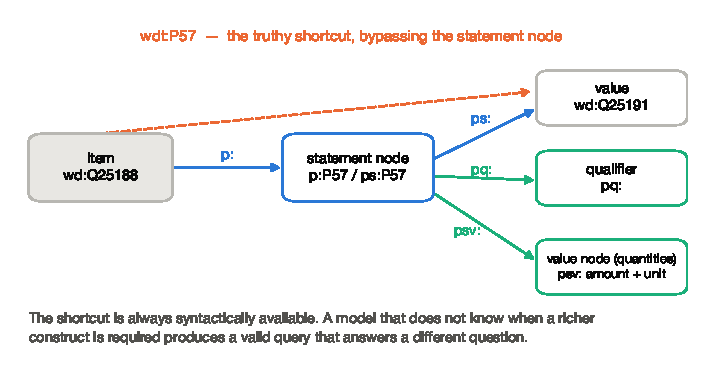
\includegraphics[width=0.88\textwidth]{figures/fig_wikidata_model.pdf}
  \caption{The Wikidata statement model.}
  \label{fig:wikidata-model}
  \tabnote{The truthy edge wdt: bypasses the statement node.
Qualifiers (pq:) and normalised value nodes (psv:) are reached
through p:/ps:.}
\end{figure}

\Cref{fig:wikidata-model} summarises these relationships.
One of them matters most here: the simpler query form is always syntactically available.
A model can use wdt: even when a statement node, qualifier or normalised value node is actually needed.
The resulting query is valid and may even return plausible results, yet it answers the wrong question.

Syntax checking cannot detect such an error; a comparison with the result of the gold query can.
Better entity linking cannot fix such an error either, because the identifiers are already correct.
For this reason, the thesis analyses structural and linking errors separately.

\subsection{SPARQL and Query Engines}

\label{sec:sparql}

SPARQL is the W3C query language for RDF, and the benchmark uses only part of it.
SPARQL matches graph patterns built from triple patterns and returns the variables selected in the SELECT clause.
The benchmark also uses FILTER for value constraints, OPTIONAL for left-join behaviour when a value may be missing, UNION for alternative patterns, aggregation with GROUP BY and HAVING, ordering and LIMIT, property paths such as the * and / operators described above, and subqueries.
Property paths matter for meaning, but they are also expensive to run.
Where they are placed and the order in which joins are evaluated can strongly affect execution time on a graph as large as Wikidata~\citep{aimonier2023joinordering}.

Two further features are specific to the Wikidata deployment.
The label service (SERVICE wikibase:label) adds human-readable labels to the identifiers in query results, and most published Wikidata queries use it.
The mwapi service lets a query call the MediaWiki API during execution, for example for full-text search.

\paragraph{Blazegraph and QLever}

The benchmark's gold queries were written for the public Wikidata Query Service, which runs on Blazegraph.
The experiments use a dedicated QLever instance instead~\citep{bast2017qlever}.
The reasons are practical: a local endpoint avoids the rate limits and timeouts of the public service and makes it easier to run thousands of queries under controlled conditions.
It also keeps the graph from changing during the experiments.

The two engines are not fully interchangeable.
Blazegraph supports named subqueries (WITH \ldots{} AS), the geospatial service wikibase:around, the mwapi service and the ``gas'' graph-traversal services; QLever does not.
QLever also applies stricter rules to AS targets and so rejects some queries that Blazegraph accepts.
As a result, around 15\,\% of the benchmark's gold queries run only on Blazegraph and are excluded from the evaluation.
The method chapter describes this issue in detail and discusses engine choice as a threat to comparability.

Real-world query use offers another point of comparison.
\citet{malyshev2018getting} analysed Wikidata Query Service logs and found that real users rely heavily on the label service and basic graph patterns, while more complex constructs are rarer.
The same comparison is made here, using the larger and more recent query-log corpus released by \citet{walter2026wdql}.
WDBench~\citep{angles2022wdbench} is a complementary benchmark built directly from public Wikidata query logs.

\section{Text-to-SPARQL and KGQA}

\subsection{Knowledge Graph Question
Answering}

\label{sec:kgqa}

Knowledge graph question answering (KGQA) means answering natural-language questions with the help of a knowledge graph.
Current research falls broadly into two approaches.
Recent surveys of large language models and knowledge graphs draw a similar line~\citep{ma2025llmkg}, as does a systematic review of the wider KGQA architecture space~\citep{perevalov2024survey}.

\paragraph{Retrieval-based
answering} treats the graph as a source to retrieve information from.
Relevant triples or subgraphs are retrieved, turned into text and given to a language model, which writes the answer directly.
This approach copes fairly well with differences in graph schema and needs no knowledge of query syntax.
The answer, however, is generated rather than computed.
It cannot be audited directly or re-run when the graph changes, and it does not scale naturally to large numbers of entities.
A question that needs aggregation over thousands of entities, for instance, cannot usually be answered from a handful of retrieved triples.

\paragraph{Semantic parsing} translates the natural-language question into an executable SPARQL
query.
The answer then comes from executing the query on the graph.
This work uses semantic parsing, because the query is an artefact that can be inspected and verified, works over any number of entities, and stays useful as the graph is updated.
The price is brittleness: one wrong identifier or one missing * can yield a query that is valid but wrong.
The experiments here measure and attribute this kind of failure.

Within semantic parsing, three system paradigms recur:

\begin{description}
\item[Fine-tuned sequence-to-sequence models]
are trained on question--query pairs and generate a query in one pass.
\item[Pipelines]
divide the task into explicit stages, typically including mention detection, linking, query generation, and execution~\citep{banerjee2024diss}.
Each stage can use a separate component or prompt.
\item[Agents]
give a model tools for exploring the graph and iteratively modifying a query.
Execution results can be used as feedback across multiple turns.
\end{description}

This thesis uses a pipeline.
Fine-tuned models need in-domain training data, have to be retrained for every knowledge graph, and cannot be built on frontier models that are only available through an API.
Agents can recover from their own mistakes, but they make many model and endpoint calls per question, and because each step depends on the one before, it is hard to tell which step caused a failure.
A pipeline keeps every stage observable, so each error can be traced to a specific stage, which is the central aim of this thesis.

\subsection{Text-to-SPARQL with Language
Models}

\label{sec:related-t2s}

The following paragraphs cover fine-tuned models, prompting, in-context learning, and agents, followed by recent schema-aware grounding methods that can complement these approaches.

\paragraph{Fine-tuned sequence-to-sequence
models}

\citet{banerjee2022modern} establish Wikidata semantic-parsing baselines with pre-trained sequence-to-sequence models.
They supply entity and relation links instead of predicting them, so the evaluation isolates query generation, and general-purpose models turn out to compete with task-specific architectures once linking is fixed.
\citet{xu2023wikisp} fine-tune LLaMA and introduce WikiWebQuestions, attributing 35.1\,\% of failures to entity linking (``the biggest source of errors'') and 17.1\,\% to the wrong property.
That attribution is re-tested here under two conditions that differ from theirs: their percentages are computed over failed examples only, and their system is fine-tuned on relatively simple questions.
When the generator is a frozen frontier model and disambiguation is close to perfect, the remaining error looks different: structure dominates, and linking contributes little.

\paragraph{Prompting and in-context
learning}

\citet{dabramo2025investigating} study in-context learning for text-to-SPARQL on benchmarks that supply gold entities and relations (so their evaluation, like \citet{banerjee2022modern}'s, isolates generation), and identify a systematic \emph{triple-flip} error: the model reverses the subject and object of a generated triple, producing a query that is valid, incorrect and often empty.
Their fix keeps several beam-search hypotheses instead of only the most probable one.
This independently supports the distinction between linking and structure drawn here.
It also connects to the empty results observed in this work: a structurally wrong query over correct identifiers often returns nothing, so an empty result can be a diagnostic signal.
Few-shot demonstrations can also teach more than surface format: \citet{shah2024implicit} show that examples which make implicit multi-hop reasoning steps visible improve generated SPARQL and Cypher queries, a more targeted use of demonstrations than the few-shot condition tested here.

\paragraph{Agentic systems}

Agentic approaches let a model explore the graph and revise a query over several steps~\citep{liu2024spinach}.
The TEXT2SPARQL'25 challenge produced several such systems: mKGQAgent~\citep{perevalov2025mkgqagent} won overall with a multilingual pipeline modelled on human reasoning; \citet{brei2025aruqula} combine ReAct-style reasoning with graph-exploration tools; and \citet{walter2025grasp} extend the approach from one knowledge graph to many.
\citet{soru2026researcher}'s self-improving agent reaches 0.22 accuracy on the 2025 DBpedia validation set and concludes that ``the bottleneck is consistently in basic-graph-pattern predicate selection, not in SPARQL syntax or modifiers''.
On a different graph and system, this supports the failure taxonomy of this work.
These systems share execution-guided revision, and the cascade used here is a deliberately minimal form of it.

\paragraph{Schema-aware grounding}

\citet{zhang2026saga}'s SAGA keeps a persistent bidirectional type state and filters candidate properties by entity type, property domain/range and expected answer type, reporting the highest F1 across nine Wikidata/Freebase settings and fewer empty results.
In other words, SAGA removes unsuitable candidates before generation.
The schema-evidence prompt tested in this work only adds schema information to the prompt as text, which the generator is free to ignore, and in the experiments here it did not improve accuracy.
The discussion chapter explains why this difference, filtering the candidate space rather than merely informing it, matters.
\citet{yang2026ggc}'s Generator--Gate--Corrector applies correction only to the questions that need it and cuts inference overhead by 45\,\%.
The selective-application experiment in this work tests the same gating idea for a different intervention and finds that it does not beat applying the intervention everywhere.
\citet{srivastava2026mars} use adaptive multi-hop retrieval that learns when to stop traversing the graph and start generating, with competitive results on three multilingual KGQA benchmarks.
Recent production-oriented systems organise text-to-SPARQL in the same way, as a pipeline of metadata indexing, prompt construction, generation and execution, which shows how much grounding and endpoint interaction matter beyond one-shot query decoding~\citep{smeros2025sparqlllm}.

\section{Entity Linking for KGQA}

\subsection{Entity Linking}

\label{sec:el-background}

Entity linking maps textual mentions to identifiers in a knowledge base.
\citet{shen2015entitylinking} describe the standard three stages: \emph{mention detection}, which finds the spans to be linked; \emph{candidate generation}, which retrieves a shortlist of possible identifiers for each mention, usually from an alias index; and \emph{candidate ranking}.
\citet{moller2022survey} show that Wikidata entity linking is shaped by conditions that ordinary systems for encyclopaedic text make little use of: a multilingual and constantly changing space of labels and aliases, a long tail of non-named entities, and the hyper-relational statement model described above, which carries more information than a plain named-entity mention.
The linking results later in the thesis should be read with this last point in mind.

\paragraph{Linking for a query is not linking in
text.}

A classic entity linker finds references to named entities in a document and connects them to knowledge-base identifiers.
It is built for running text.
A text-to-SPARQL pipeline needs something different, because a query may require identifiers for relations (P57, director), type constraints (Q5, human), units and aggregation concepts.
Many of these never appear as named entities in the question.
“How many female directors won an Oscar after 2000?” may require identifiers for instance of, human, sex or gender, female, award received and director, although several of these concepts are not explicit spans in the text.
A linker that starts from mention detection in the text cannot find a concept the question does not state.
This is a mismatch between the task these systems were built for and the task they face here, not necessarily a flaw in their implementation.
It helps explain the large differences in the linker comparison between text-driven end-to-end linkers and approaches that reason over candidates retrieved for the vocabulary a query needs.
These results should not be read as a general judgement on end-to-end linking systems.

\subsection{Entity Linking Paradigms}

\label{sec:related-linking}

The following three paradigms correspond to the linking approaches evaluated here.
The section closes with how linkers should be evaluated so that they can be compared fairly.

\paragraph{Fine-tuned end-to-end
linking}

\citet{wu2020blink} introduced BLINK, a two-stage architecture in which a bi-encoder retrieves candidates by dense vector similarity and a cross-encoder re-ranks them.
It is trained on Wikipedia hyperlinks and transfers zero-shot to unseen entities.
\citet{li2020elq} adapt this approach to questions with ELQ, which detects and links mentions in a single pass over the question, with efficiency as a central design goal.
\citet{ayoola2022refined} propose ReFinED, which performs mention detection, fine-grained typing and disambiguation in one pass over a document and scales to the full Wikidata entity set.

All three systems are trained on running text and detect mentions in that text.
As discussed above, this is not the same as supplying the broader vocabulary a SPARQL query needs, and their results in the linker comparison should be read with this mismatch in mind.

\paragraph{Zero-shot bi-encoder
retrieval}

GLiNER is a lightweight named-entity recognition model that compares text spans with descriptions of entity types, so it can recognise types it was not trained on.
\citet{stepanov2026glinker} extend its bi-encoder variant to large label spaces and introduce GLiNKER as an entity-linking framework.
Its main advantages here are that it needs no task-specific training and scales to Wikidata's large label space.
Its drawback is typical of bi-encoders: the mention and each candidate are encoded separately, which makes retrieval fast but rules out a detailed comparison between them, so similar candidates are harder to tell apart than when they are ranked jointly with the question.

\paragraph{Reasoning over retrieved
candidates}

The third paradigm retrieves candidates from an alias index and asks a language model to choose among them, using the question as context.
\citet{alekseev2025querybased} evaluate this approach inside a multi-stage Wikidata pipeline.
They compare reasoning-based selection with fine-tuned linking and argue for query-based KGQA on complex and temporal questions.
Theirs is the published work closest to the pipeline evaluated here, and the end of this chapter positions this thesis against it explicitly.

\citet{vollmers2025evaluation} evaluate entity and relation linking specifically for KGQA.
They report that linkers based on language models clearly outperform other approaches, especially in recall.
In their comparison, traditional systems reach higher precision but much lower recall.
They also draw a conclusion that bears directly on the design used here: high recall, even at some cost in precision, can give better end-to-end performance, because the downstream model tolerates noisy candidate sets.

The same pattern appears here, on a different benchmark and with differently constructed ground truth.
It also explains the candidate-pool design used here: retrieval deliberately admits candidates generously, and the disambiguation stage is responsible for choosing the right one with the full question as context.

\paragraph{Evaluation protocol}

\citet{bast2023fairel} point out that published end-to-end entity-linking results are often hard to compare, because systems differ in what they count as a mention, how they score partial overlaps and which knowledge-base version they use.
They propose an evaluation framework that controls these choices.
The linking comparison here follows the same discipline: all four linkers are evaluated on identical rows, against identical ground truth, with identical scoring.
The ground truth comes from the benchmark's own annotated queries, not from an external linker's index.

\section{Benchmarks, Evaluation, and Research
Gap}

\subsection{Benchmarks and Evaluation
Practice}

\label{sec:related-eval}

\paragraph{The benchmark used here}

\citet{benamor2025instruct} introduce Instruct-to-SPARQL, built by crawling Wikidata tutorial and example pages and pairing the queries found there with generated instructions and complexity labels.
Two of its properties matter here.
Because it comes from documentation and community examples rather than templates, it contains a wide range of Wikidata-specific idioms (qualifiers, statement nodes, the label service), which suits a study of structural competence.
And, as the authors state, it comes with no entity-linking strategy, leaving grounding to the system.
\citet{dubey2019lcquad2} remains one of the most widely used Wikidata KGQA benchmarks and offers a point of comparison for scale and construction.

\paragraph{The comparability problem}

Published text-to-SPARQL results are hard to compare directly: studies use different graph snapshots, metrics that share a name but not a definition, and gold queries that may no longer execute.
This is part of a wider benchmark-design problem in KGQA: datasets differ in how they construct questions, annotate logical forms and define complexity, so reported improvements may not carry over to other benchmarks or graph snapshots~\citep{steinmetz2021kgqabenchmarks}.
\citet{taghzouti2026t2smetrics} document this fragmentation and propose a unified evaluation library, which itself shows that consistency is still an open issue.
For this reason, the benchmark authors' generated queries are re-executed here against the same snapshot, fair-set definition and metric as every other system, and published scores are not compared directly.

\paragraph{Contamination and
memorisation}

A model that saw a benchmark's gold queries during pre-training may partly reproduce them from memory.
\citet{gashkov2025memorization} show that this can affect reported performance on QALD and LC-QuAD.
Instead of assuming that the frozen frontier models are or are not contaminated, this work measures the effect directly.
Identifiers, literals and variable names are removed from every generated query, and the remaining structure is compared with the benchmark's reference queries.
A model that had memorised the benchmark would often reproduce them almost exactly.

\paragraph{External validity}

A benchmark's mix of constructs does not necessarily reflect what users actually ask.
\citet{malyshev2018getting} established the practice of comparing benchmark constructs with Wikidata Query Service logs, and \citet{walter2026wdql} released a much larger derived resource of 335,000 question--query pairs for the same purpose.
It is used here to check whether the Wikidata idioms under study are a property of the benchmark or of real-world use.

\subsection{Positioning of This Work}

\label{sec:positioning}

\paragraph{Established components}

The pipeline builds on two established mechanisms: reasoning-based disambiguation over retrieved candidates, studied by \citet{alekseev2025querybased} (who compare it with fine-tuned linking in a multi-stage Wikidata pipeline) and \citet{vollmers2025evaluation}; and execution-guided revision, established in the agentic systems discussed above.
The cascade used here is a minimal, single-round form of execution feedback, added because the measurements showed remaining headroom.

\paragraph{What differs here}

The linking comparison evaluates four paradigms on the same rows, ground truth and candidate pools, with the gold standard taken from the benchmark's own annotated queries.
Error is attributed to individual stages, with backbone dependence measured separately for each, instead of being reduced to one end-to-end score.
Interventions are controlled by changing only the generation prompt, and four directions are tested: generic guidance, schema evidence, selective guidance and a closed vocabulary.
External validity is checked against real query-log usage in both directions.

\paragraph{Framing}

The contribution is primarily measurement and attribution: finding where a frozen-model pipeline fails, identifying which component is the main constraint, and introducing one mechanism that follows directly from that evidence.
